\chapter{Задание 1. Жёсткие фильтры}
\label{ch:chap2}

\definecolor{codegreen}{rgb}{0,0.6,0}
\definecolor{codegray}{rgb}{0.5,0.5,0.5}
\definecolor{codepurple}{rgb}{0.58,0,0.82}
\definecolor{backcolour}{rgb}{0.95,0.95,0.92}

\lstdefinestyle{mystyle}{
    backgroundcolor=\color{backcolour},   
    commentstyle=\color{codegreen},
    keywordstyle=\color{magenta},
    numberstyle=\tiny\color{codegray},
    stringstyle=\color{codepurple},
    basicstyle=\ttfamily\footnotesize,
    breakatwhitespace=false,         
    breaklines=true,                 
    captionpos=b,                    
    keepspaces=true,                 
    numbers=left,                    
    numbersep=5pt,                  
    showspaces=false,                
    showstringspaces=false,
    showtabs=false,                  
    tabsize=2
}
\lstset{style=mystyle}


% \textit{NB.} - В этом задании мы используем унитарное преобразование Фурье к угловой частоте $\omega$, оно будет выглядеть следующим образом: 


Для начала задаём константы $a, b, c, d, t_1, t_2$, что $t_1 < t_2$, После составляем функцию:
$$
g(t) = \begin{cases}
        a, t\in[t_1 ; t_2] \\
        0, t\in[else]
       \end{cases}
$$
Также задаём большой интервал времени $T$ и маленький шаг дискретизации $dt$. На основе всего зашумлённая версия сигнала будет выглядеть так:
$$
\texttt{u = g + b*(rand(size(t))-0.5) + c*sin(d*t);}
$$

\section{Убираем высокие частоты}

Берём $d=c=0$. Тогда в этом пункте мы будем работать со следующей версией шумного сигнала:
$$
\texttt{u = g + b*(rand(size(t))-0.5)}
$$\dots из чего сразу следует, что у нас добавляется только "случайный" шум.

\newpage
\subsection{Фурье-образ сигнала u}

\begin{figure}[ht]
    \centering
    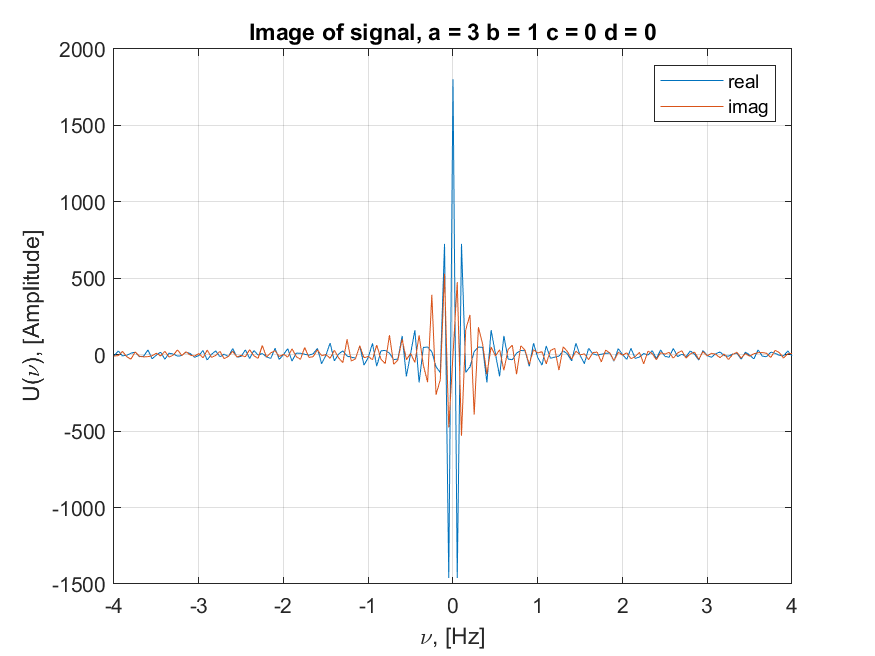
\includegraphics[width=0.6\textwidth]{image_a=3_b=1_c=0_d=0.png}
    \caption{Фурье-образ зашумлённого сигнала}
\end{figure}

\begin{figure}[ht]
    \centering
    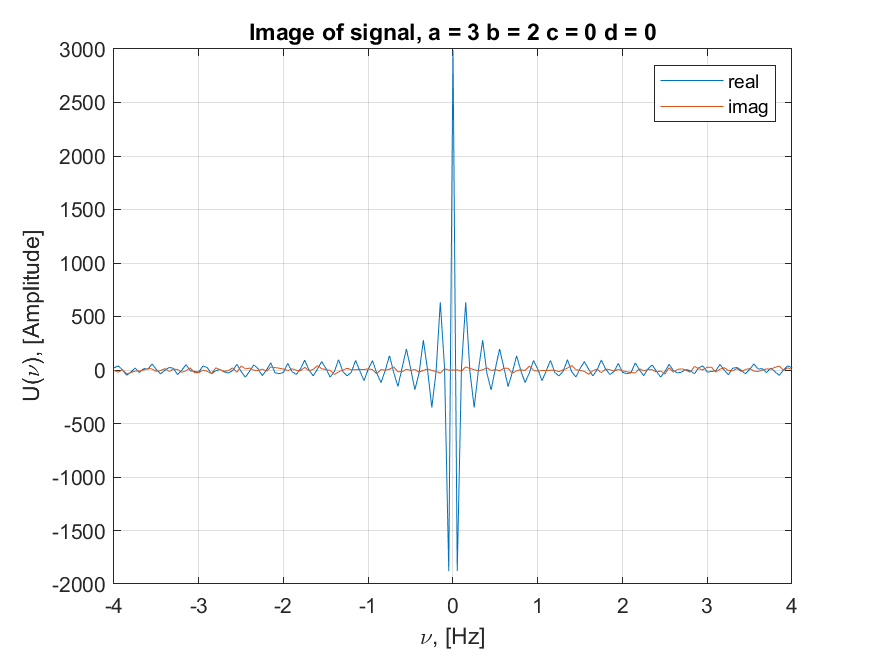
\includegraphics[width=0.6\textwidth]{image_a=3_b=2_c=0_d=0.png}
    \caption{Фурье-образ зашумлённого сигнала}
\end{figure}

\begin{figure}[ht]
    \centering
    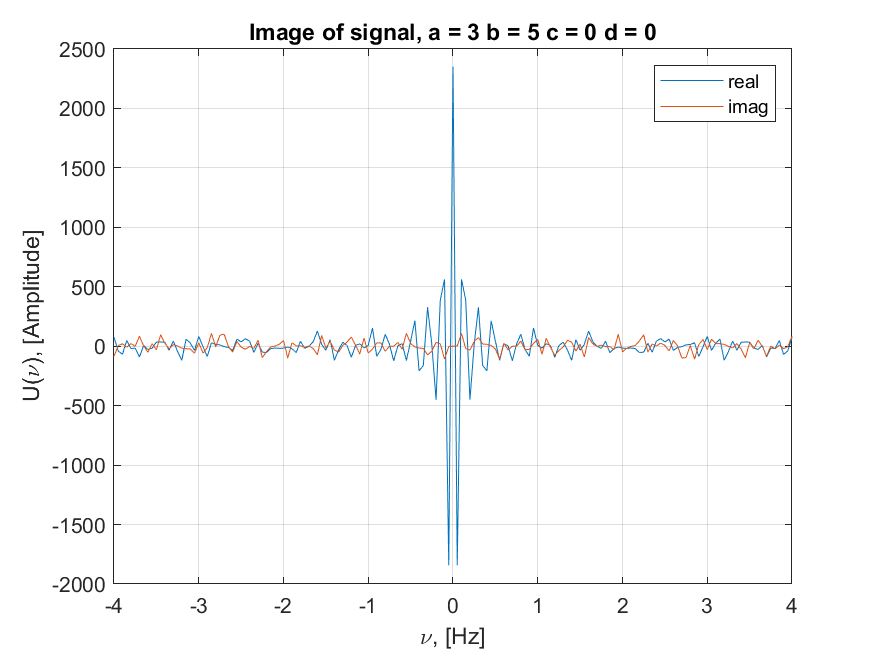
\includegraphics[width=0.6\textwidth]{image_a=3_b=5_c=0_d=0.png}
    \caption{Фурье-образ зашумлённого сигнала}
\end{figure}

\begin{figure}[ht]
    \centering
    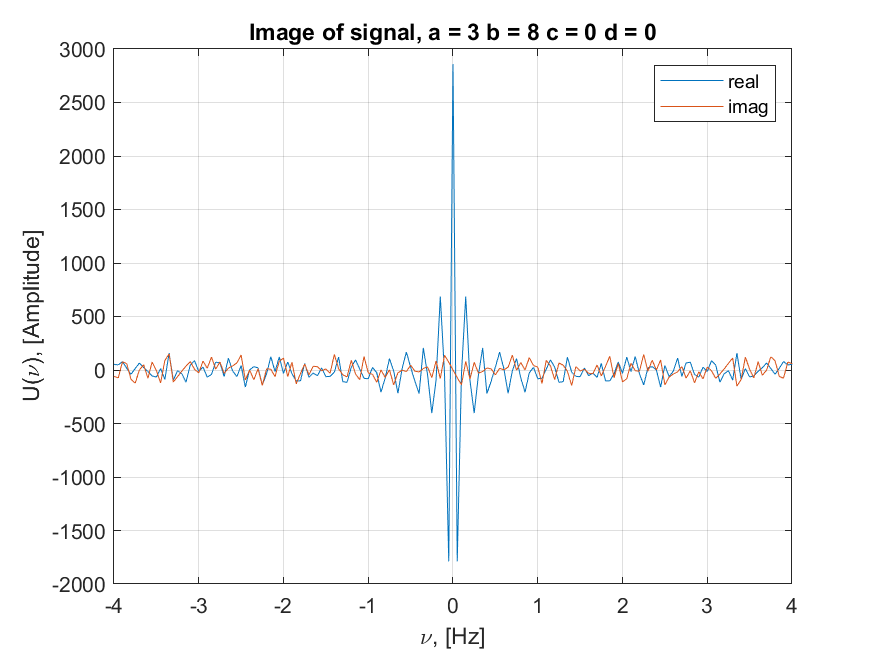
\includegraphics[width=0.6\textwidth]{image_a=3_b=8_c=0_d=0.png}
    \caption{Фурье-образ зашумлённого сигнала}
\end{figure}

\newpage
\subsection{Применяем фильтр}
В нашем случае ступенька фильтра будет около середины, потому что мы сохраняем нижние частоты, а они сосредоточены около начала графика. Будем применять разные диапазоны фильтра:

\begin{figure}[ht]
    \centering
    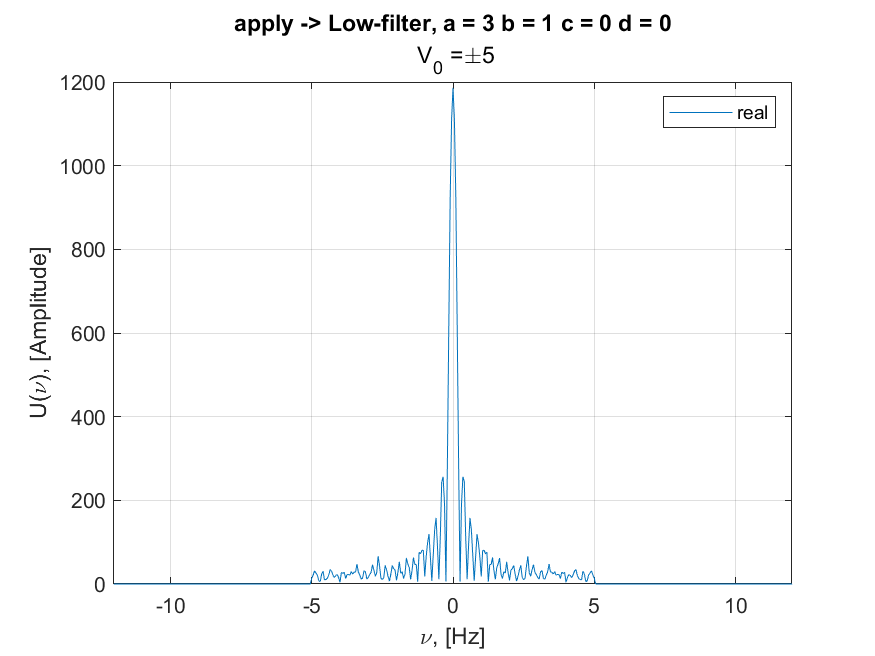
\includegraphics[width=0.6\textwidth]{applied_filter_a=3_b=1_c=0_d=0.png}
    \caption{Применили фильтр нижних частот}
\end{figure}

\begin{figure}[ht]
    \centering
    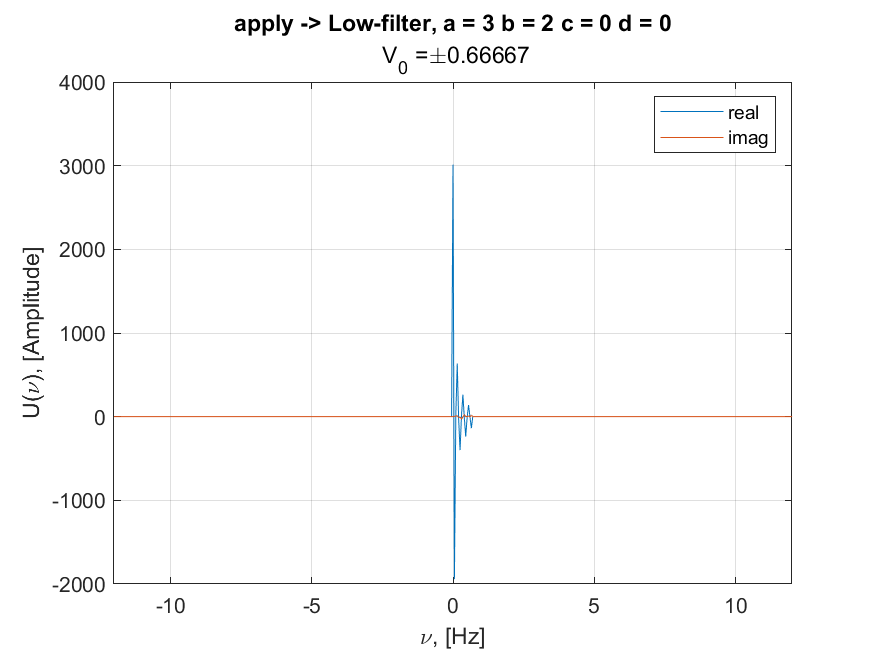
\includegraphics[width=0.6\textwidth]{applied_filter_a=3_b=2_c=0_d=0.png}
    \caption{Применили фильтр нижних частот}
\end{figure}

\begin{figure}[ht]
    \centering
    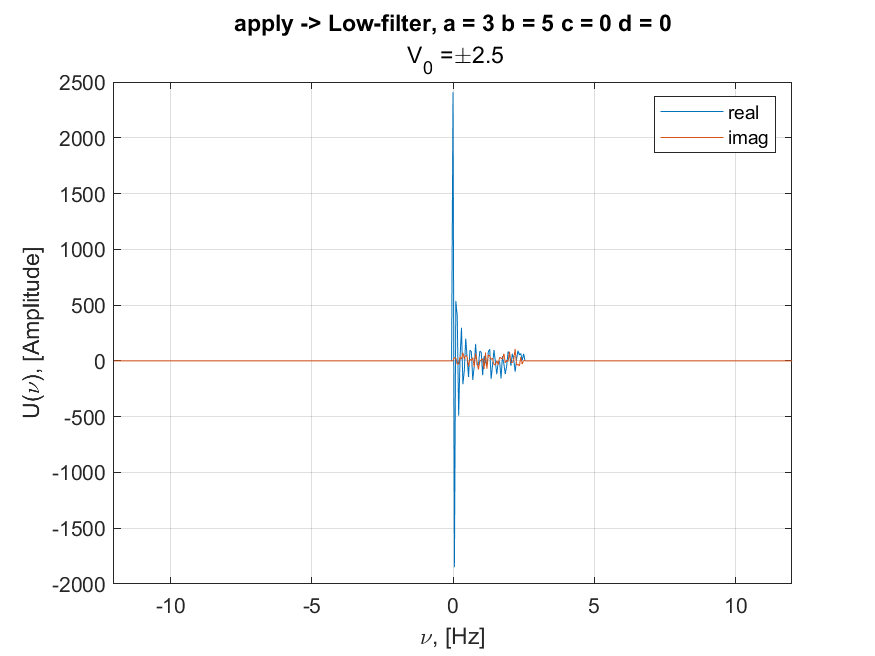
\includegraphics[width=0.6\textwidth]{applied_filter_a=3_b=5_c=0_d=0.png}
    \caption{Применили фильтр нижних частот}
\end{figure}

\begin{figure}[ht]
    \centering
    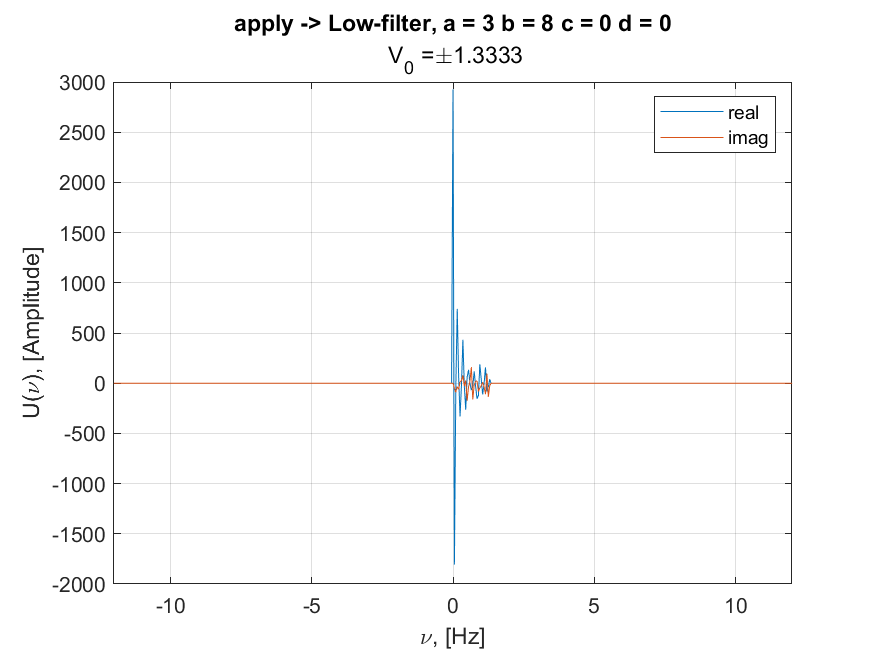
\includegraphics[width=0.6\textwidth]{applied_filter_a=3_b=8_c=0_d=0.png}
    \caption{Применили фильтр нижних частот}
\end{figure}

\newpage
\subsection{Возвращаемся к очищенному сигналу}

\begin{figure}[ht]
    \centering
    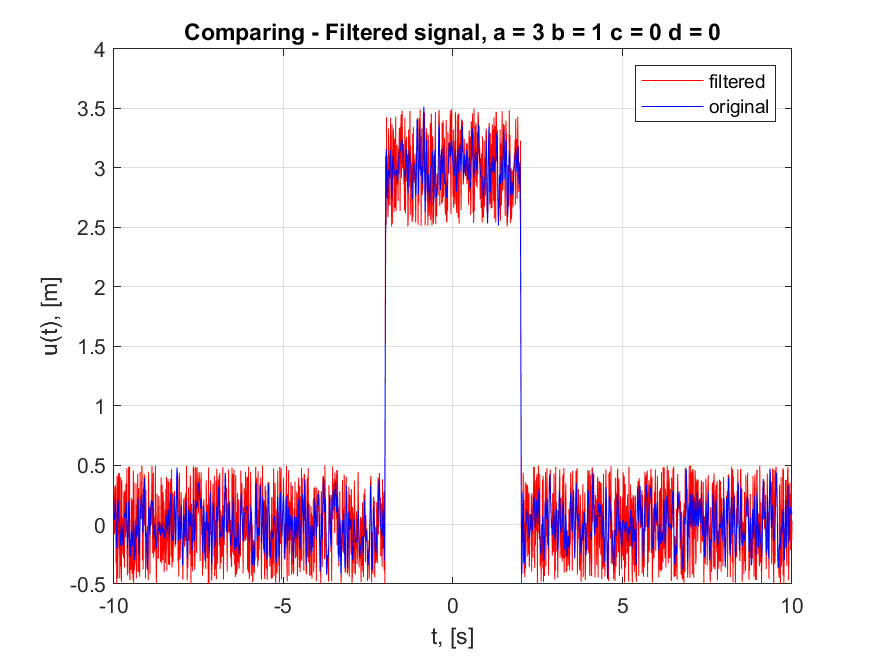
\includegraphics[width=0.6\textwidth]{pure_signal_a=3_b=1_c=0_d=0.png}
    \caption{Применили обратное преобразование Фурье}
\end{figure}

\begin{figure}[ht]
    \centering
    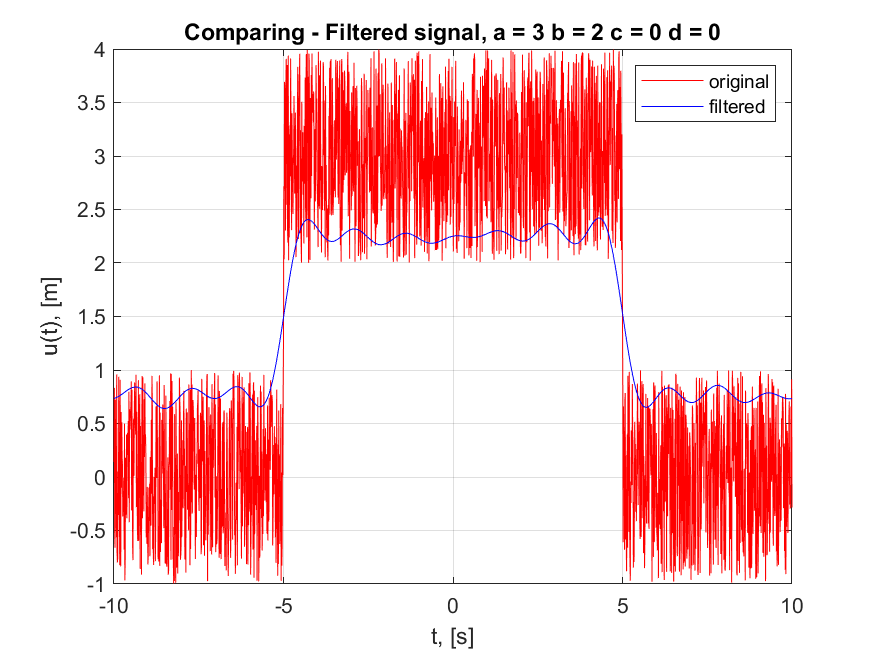
\includegraphics[width=0.6\textwidth]{pure_signal_a=3_b=2_c=0_d=0.png}
    \caption{Применили обратное преобразование Фурье}
\end{figure}

\begin{figure}[ht]
    \centering
    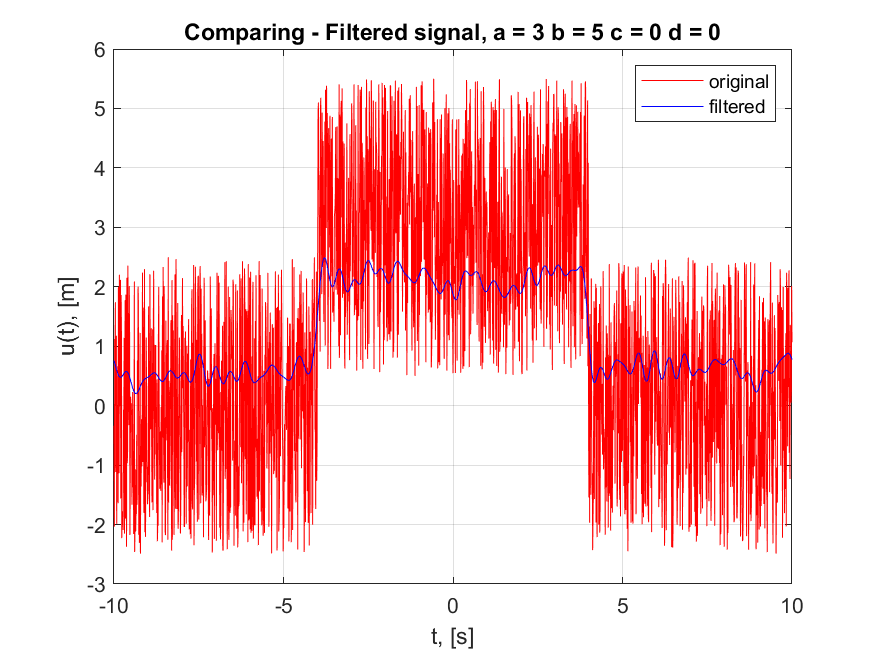
\includegraphics[width=0.6\textwidth]{pure_signal_a=3_b=5_c=0_d=0.png}
    \caption{Применили обратное преобразование Фурье}
\end{figure}

\begin{figure}[ht]
    \centering
    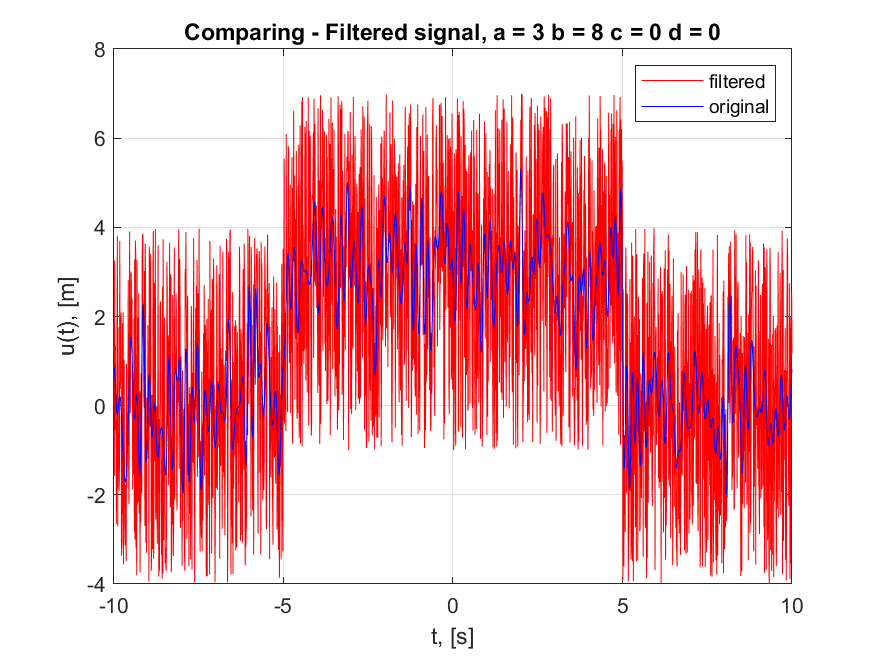
\includegraphics[width=0.6\textwidth]{pure_signal_a=3_b=8_c=0_d=0.png}
    \caption{Применили обратное преобразование Фурье}
\end{figure}

\newpage
\subsection{Выводы}

При увеличении $b$ мы добавляем больше сбвига амплитуд в исходную синусоиду, что усложняет дальнешую фильтрацию и возвращение
 к исходной функции, поэтому при фильтрации с бОльшой $b$ очищенная функция была "неуверена" в себе.
Также очевидно, при большем диапазоне фильтра мы оставляем больше частот, а значит и отфильтрованная функция будет больше колебаться, т.е. опять "неуверена" в себе. Поэтому оптимальный случай для фильтрации таким фильтром - небольшой $b$ и небольшой срез.

\section{Убираем специфические частоты}

Выберем все параметры $b, c, d$ ненулевыми. Теперь мы уже имеем дело с двумя компонентами шума - случайным и гармоническим. Соответственно, чтобы убрать обе компоненты, надо применить два фильтра, один из них мы уже нашли в пункте до.
\newpage
\subsection{Фурье-образ сигнала u}


\begin{figure}[ht]
    \centering
    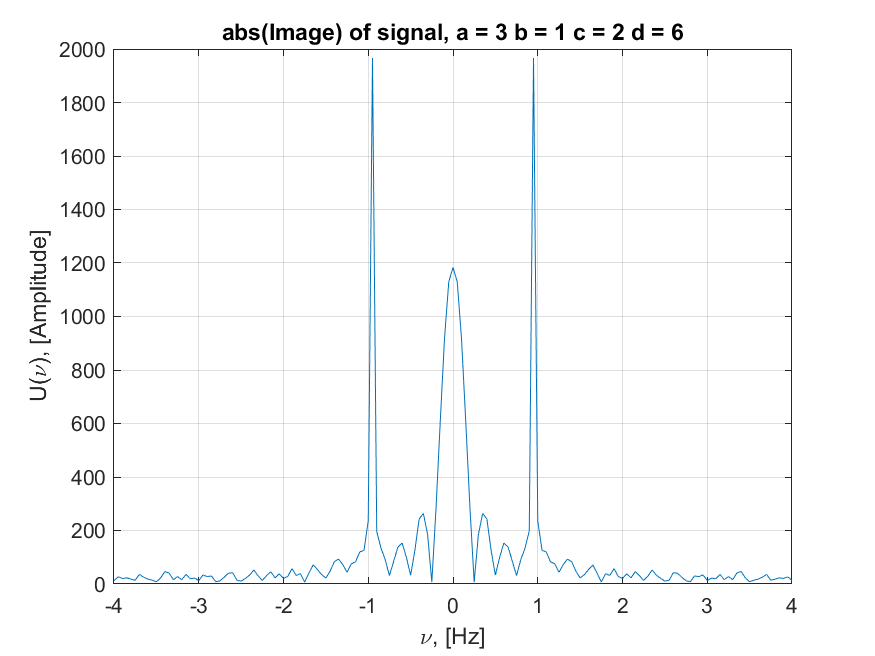
\includegraphics[width=0.6\textwidth]{abs_image_a=3_b=1_c=2_d=6.png}
    \caption{Фурье-образ зашумлённого сигнала}
\end{figure}

\begin{figure}[ht]
    \centering
    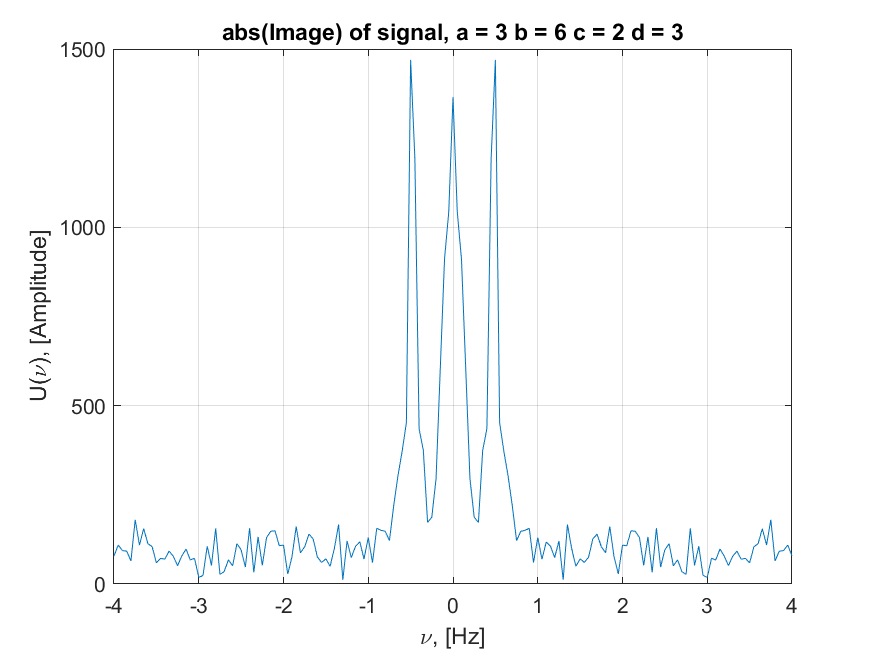
\includegraphics[width=0.6\textwidth]{abs_image_a=3_b=6_c=2_d=3.png}
    \caption{Фурье-образ зашумлённого сигнала}
\end{figure}

\begin{figure}[ht]
    \centering
    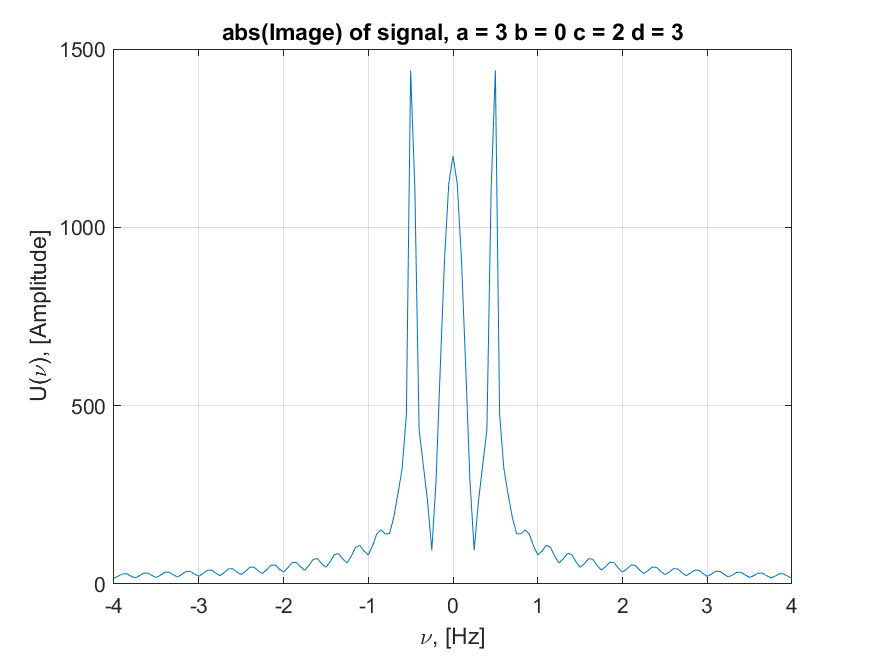
\includegraphics[width=0.6\textwidth]{abs_image_a=3_b=0_c=2_d=3.png}
    \caption{Фурье-образ зашумлённого сигнала}
\end{figure}

\begin{figure}[ht]
    \centering
    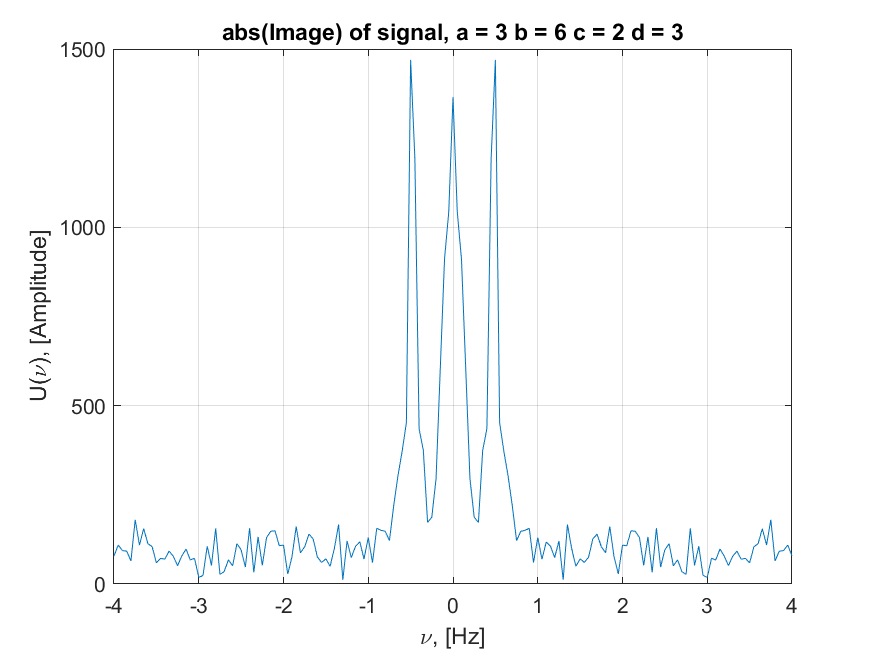
\includegraphics[width=0.6\textwidth]{abs_image_a=3_b=6_c=2_d=3.png}
    \caption{Фурье-образ зашумлённого сигнала}
\end{figure}

\newpage
\subsection{Применяем фильтр}
В данном случае далеко слишком начало пределов фильтра не стоит ставить - иначе сигнал совсем уж плохо отфильтруется.
\begin{figure}[ht]
    \centering
    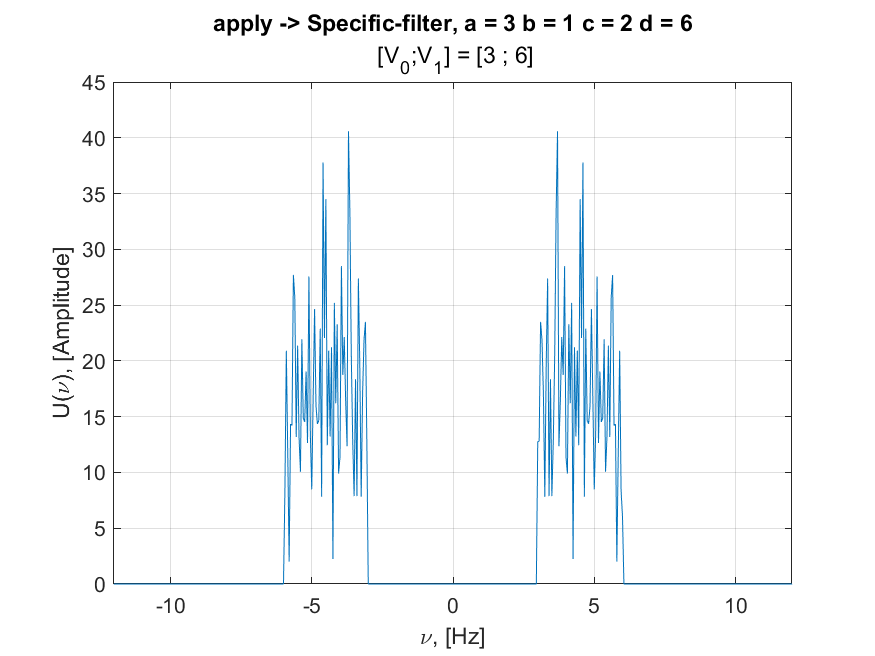
\includegraphics[width=0.6\textwidth]{applied_filter_a=3_b=1_c=2_d=6.png}
    \caption{Применили специфический фильтр}
\end{figure}

\begin{figure}[ht]
    \centering
    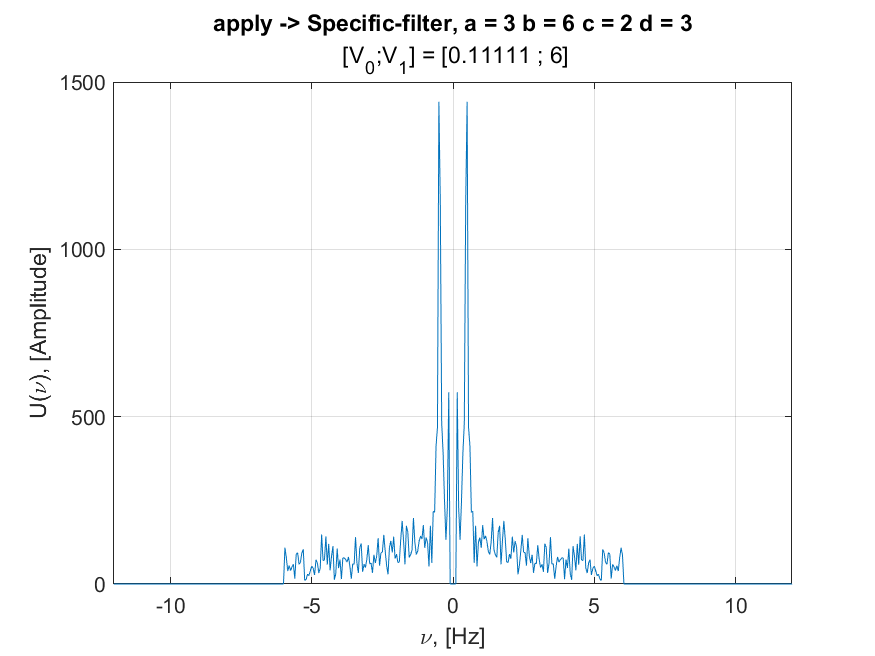
\includegraphics[width=0.6\textwidth]{applied_filter_a=3_b=6_c=2_d=3.png}
    \caption{Применили специфический фильтр}
\end{figure}

\begin{figure}[ht]
    \centering
    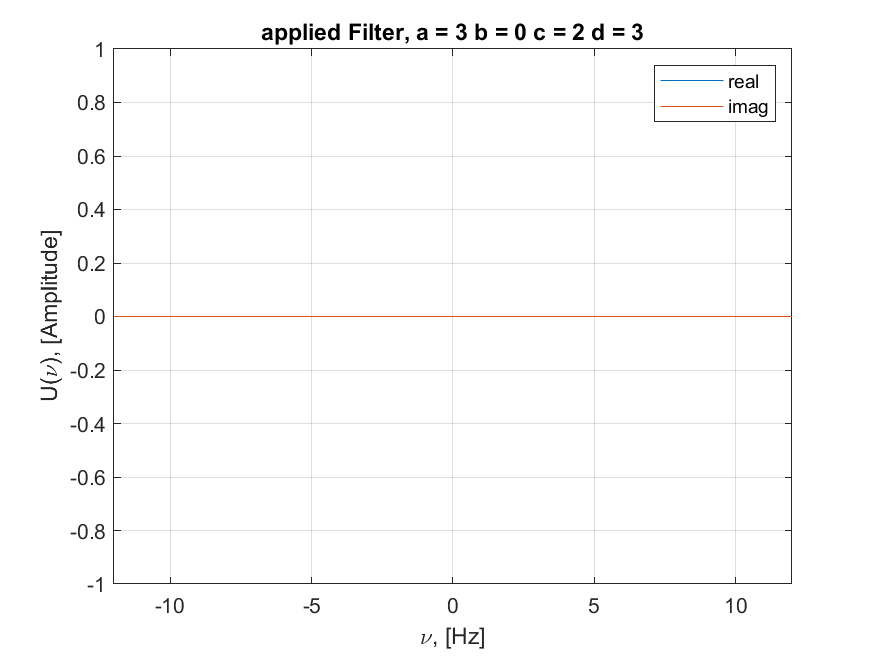
\includegraphics[width=0.6\textwidth]{applied_filter_a=3_b=0_c=2_d=3.png}
    \caption{Применили специфический фильтр}
\end{figure}

\begin{figure}[ht]
    \centering
    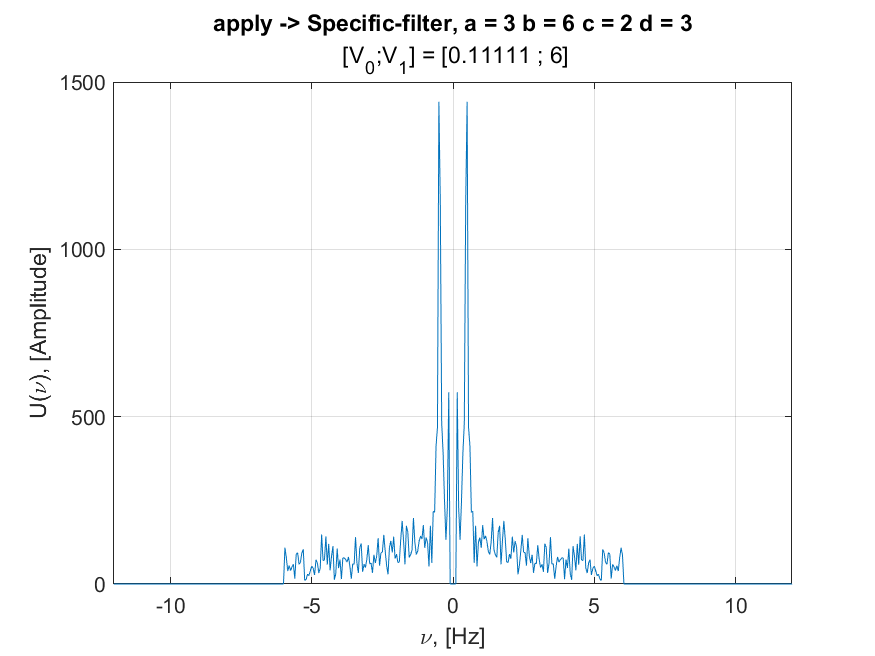
\includegraphics[width=0.6\textwidth]{applied_filter_a=3_b=6_c=2_d=3.png}
    \caption{Применили специфический фильтр}
\end{figure}

\newpage
\newpage
\subsection{Возвращаемся к очищенному сигналу}
Применяем обратное преобразование Фурье, а потом сравниваем с оригинальным сигналом\dots

\begin{figure}[ht]
    \centering
    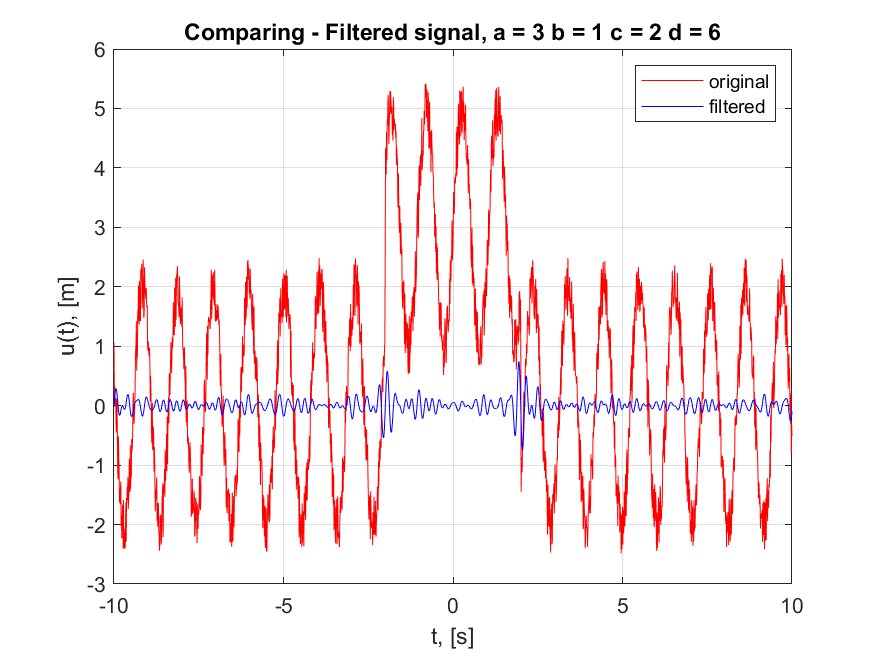
\includegraphics[width=0.6\textwidth]{pure_signal_a=3_b=1_c=2_d=6.png}
    \caption{Делаем обратное преобразование Фурье}
\end{figure}

\begin{figure}[ht]
    \centering
    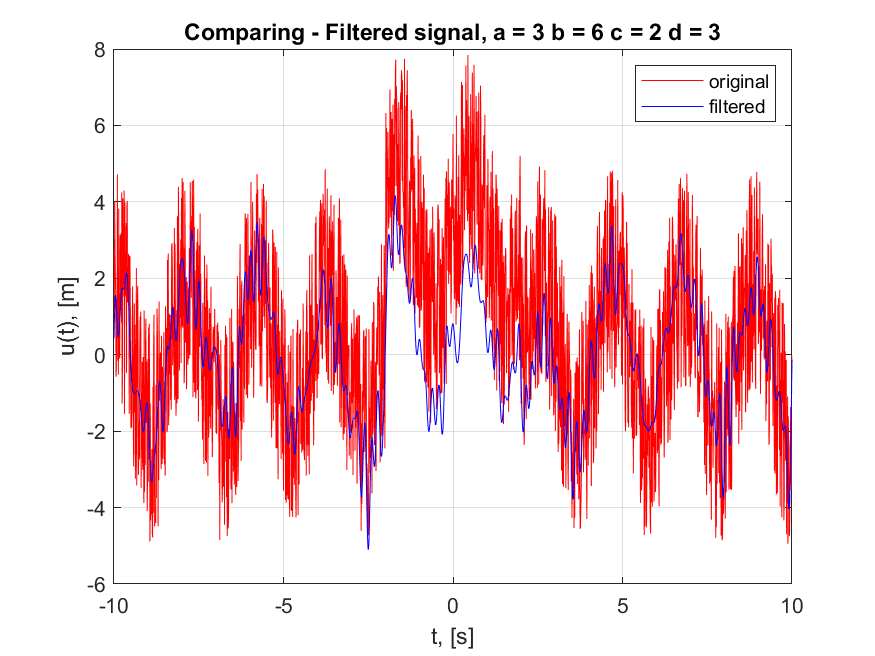
\includegraphics[width=0.6\textwidth]{pure_signal_a=3_b=6_c=2_d=3.png}
    \caption{Делаем обратное преобразование Фурье}
\end{figure}

\begin{figure}[ht]
    \centering
    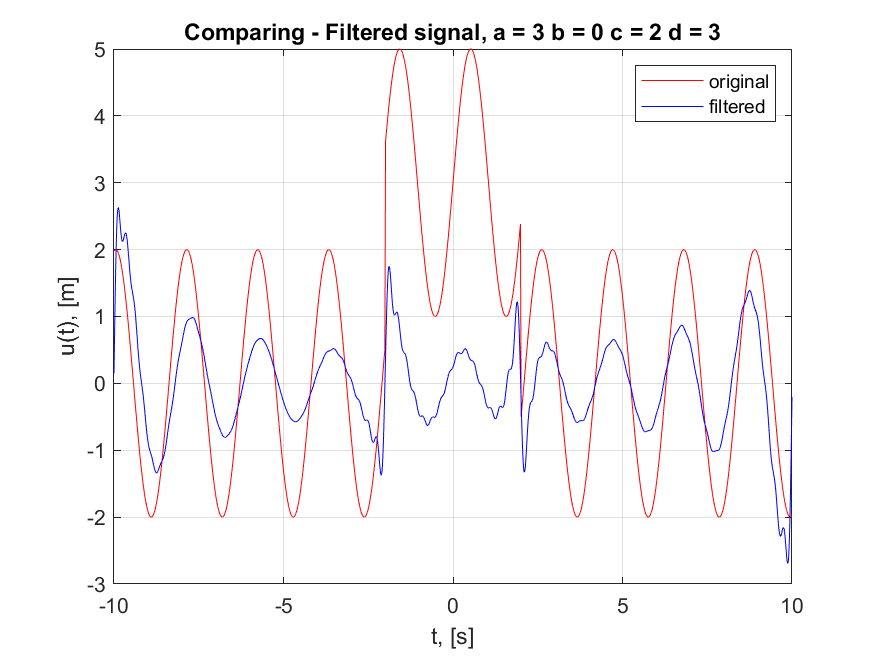
\includegraphics[width=0.6\textwidth]{pure_signal_a=3_b=0_c=2_d=3.png}
    \caption{Делаем обратное преобразование Фурье}
\end{figure}

\begin{figure}[ht]
    \centering
    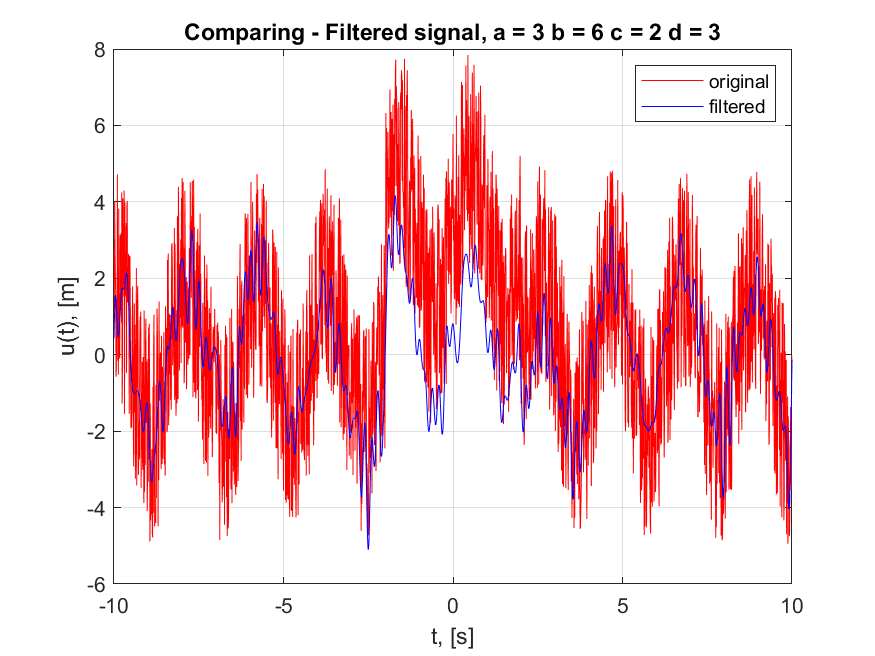
\includegraphics[width=0.6\textwidth]{pure_signal_a=3_b=6_c=2_d=3.png}
    \caption{Делаем обратное преобразование Фурье}
\end{figure}

\newpage
\subsection{Выводы}

Из формулы зашумленного сигнала понятно, что компонента $b$ отвечает за случайный шум, а $c$ и $d$ - за
гармонический, при этом $c$ - амплитуда, а $d$ - частота. Чем меньше шума было внесено в функцию, тем лучше будет получаться
его убрать. Но даже при довольно больших значениях параметров $b, c, d$ удалось убрать шум,
не сильно исказив исходную функцию. И так получилось, что только *не* срезав достаточно низких частот, мы хорошо приближаемся к исходной гладкой функции.

\newpage
\section{Убираем низкие частоты?}

Рассмотрим фильтр, который обнуляет Фурье-образ на всех частотах в некоторой окрестности точки $\nu = 0$. 
Пропустим сигнал через такой фильтр и оценим результат.

\newpage
\subsection{Фурье-образ сигнала u}


\begin{figure}[ht]
    \centering
    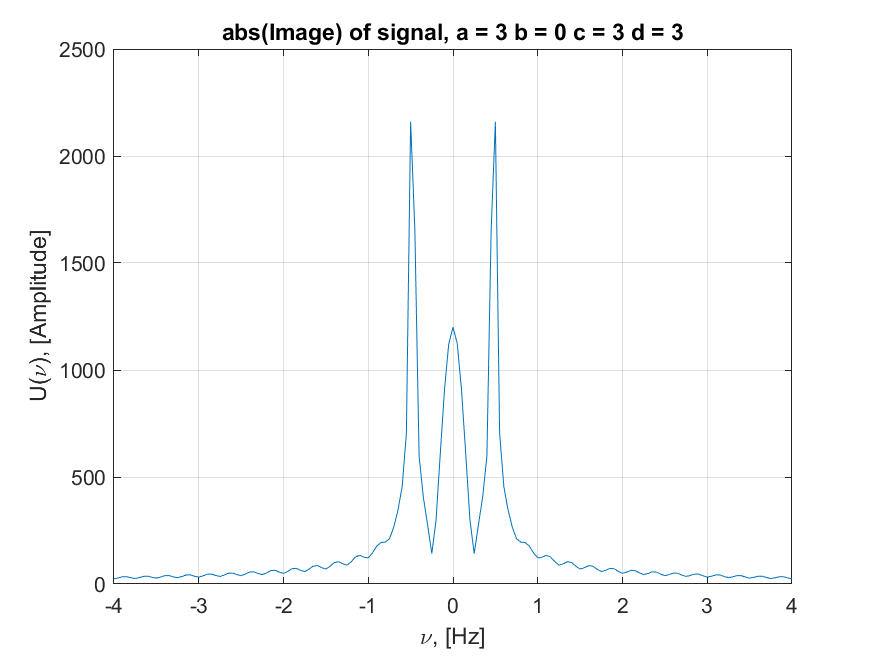
\includegraphics[width=0.6\textwidth]{abs_image_a=3_b=0_c=3_d=3.png}
    \caption{Фурье-образ зашумлённого сигнала}
\end{figure}

\begin{figure}[ht]
    \centering
    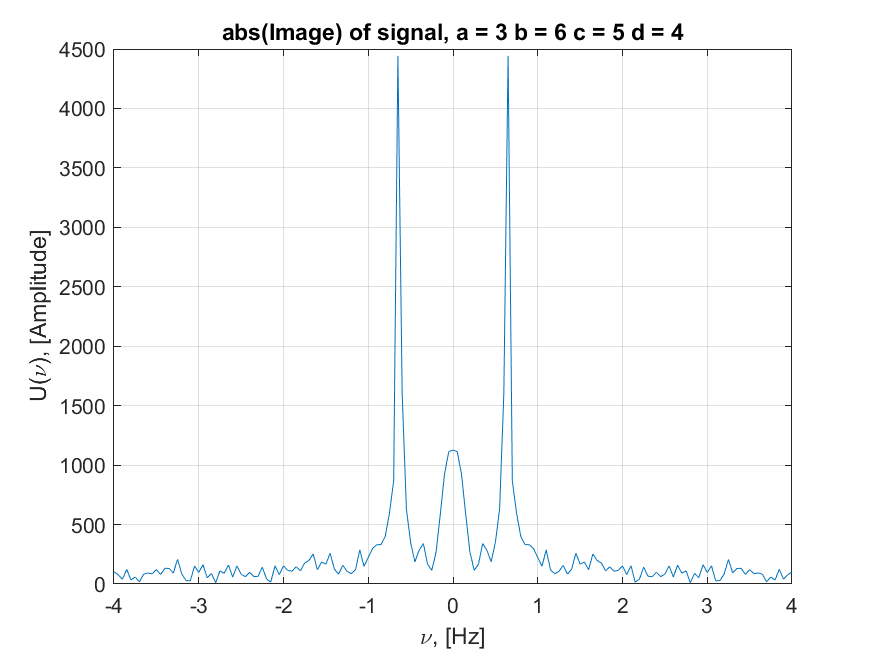
\includegraphics[width=0.6\textwidth]{abs_image_a=3_b=6_c=5_d=4.png}
    \caption{Фурье-образ зашумлённого сигнала}
\end{figure}


\newpage
\subsection{Применяем фильтр}
Текст.
\begin{figure}[ht]
    \centering
    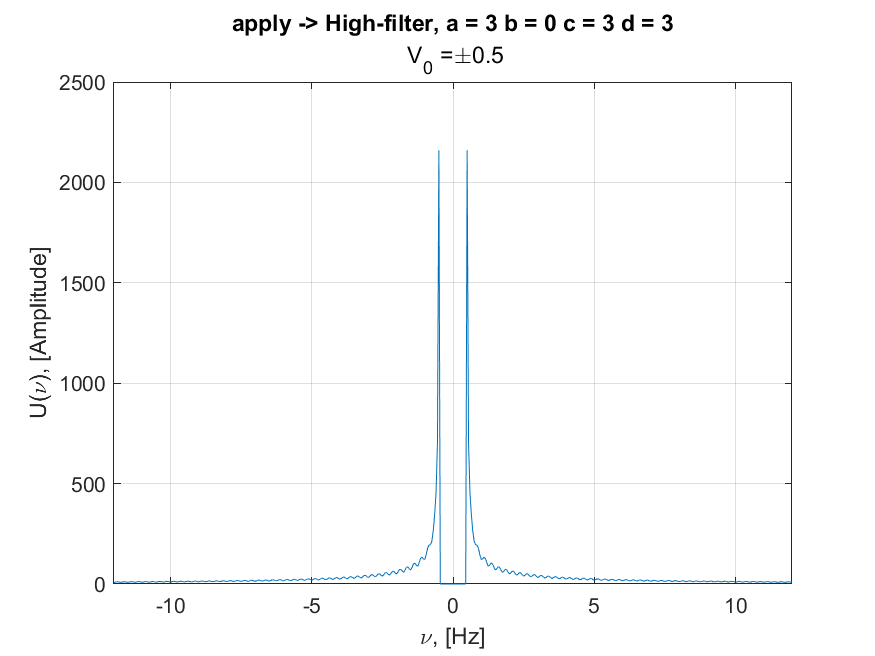
\includegraphics[width=0.6\textwidth]{applied_filter_a=3_b=0_c=3_d=3.png}
    \caption{Применяем фильтр высоких частот}
\end{figure}

\begin{figure}[ht]
    \centering
    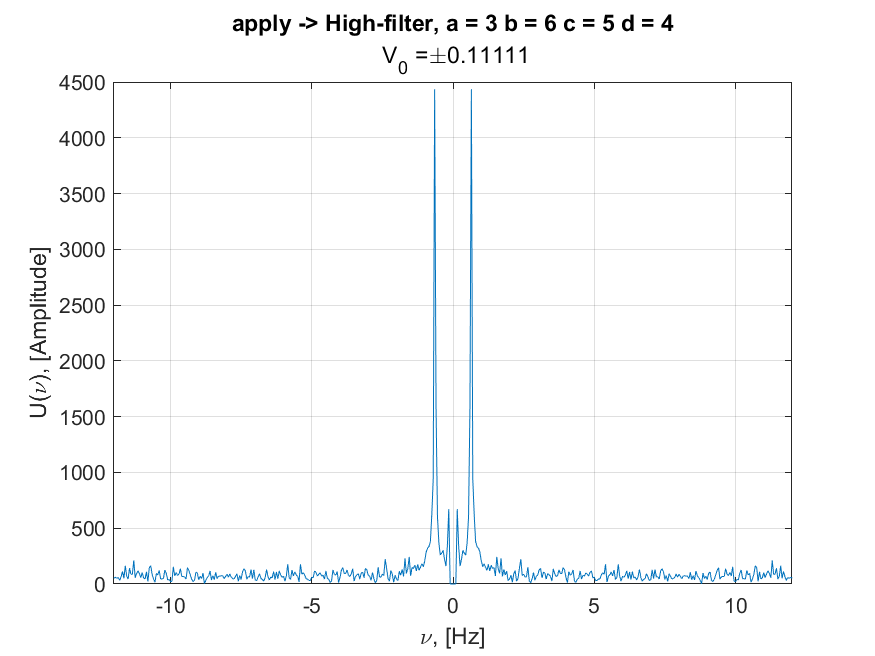
\includegraphics[width=0.6\textwidth]{applied_filter_a=3_b=6_c=5_d=4.png}
    \caption{Применяем фильтр высоких частот}
\end{figure}

\newpage
\newpage
\subsection{Возвращаемся к очищенному сигналу}
Применяем обратное преобразование Фурье, а потом сравниваем с оригинальным сигналом\dots

\begin{figure}[ht]
    \centering
    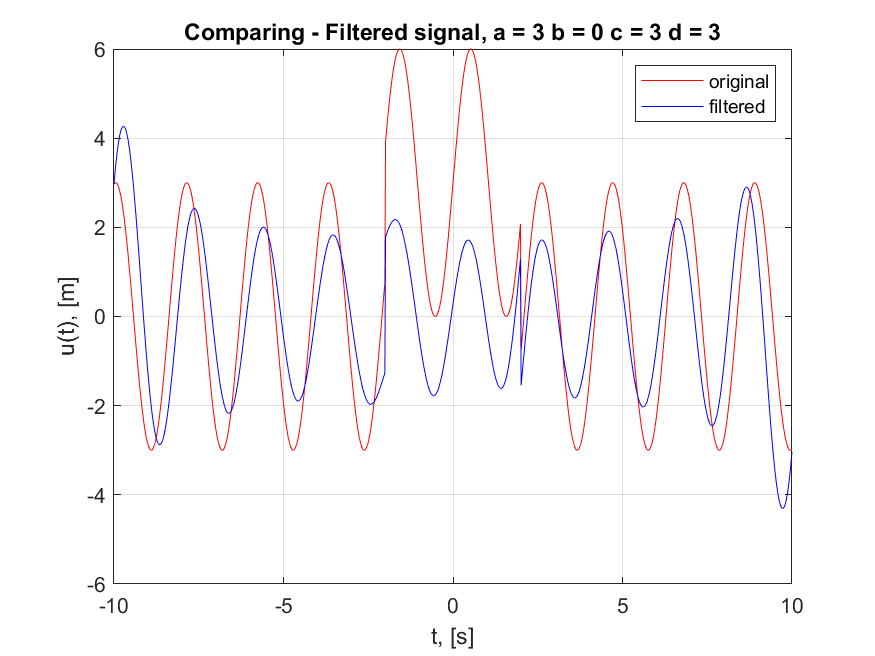
\includegraphics[width=0.6\textwidth]{pure_signal_a=3_b=0_c=3_d=3.png}
    \caption{Применяем обратное преобразование Фурье}
\end{figure}

\begin{figure}[ht]
    \centering
    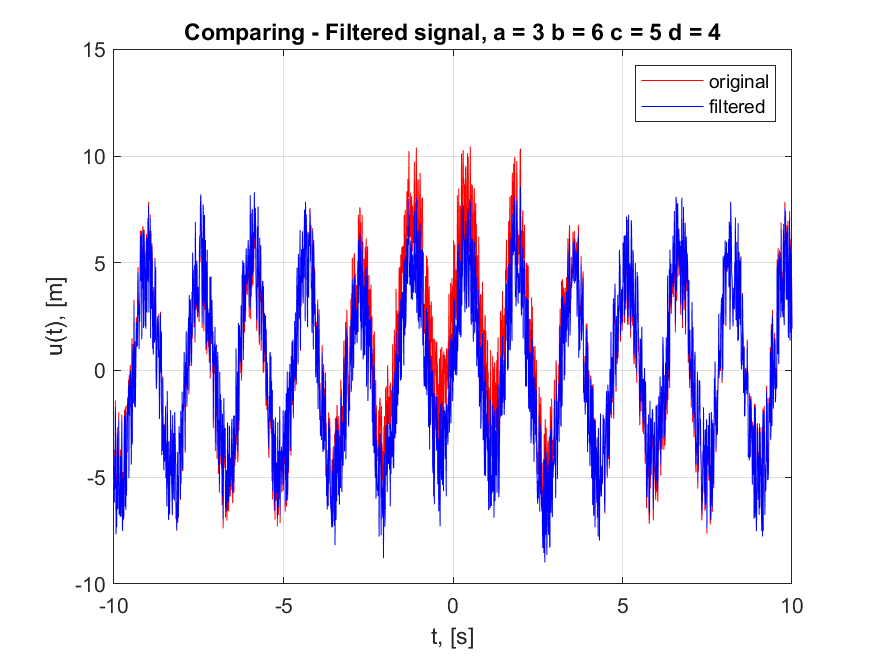
\includegraphics[width=0.6\textwidth]{pure_signal_a=3_b=6_c=5_d=4.png}
    \caption{Применяем обратное преобразование Фурье}
\end{figure}

\newpage
\subsection{Выводы}
Видно, что от исходной функции остался только шум, и это логично, ведь мы убрали низкие частоты, которые, в большинстве, 
и соответствовали самой функции. Амплитуда шума как будто осталась неизменной, что ещё раз подтверждает нашу гипотезу. Однако, если взять слишком малый срез, то функция почти будет подобать оригинальной(второй случай).

\endinput